%&tex

\chapter{Modelling the problem}\label{chp:modelling}

In this chapter we formally define a possible model for the mobile robots self-driving problem.  We
first present this problem as an imitation learning through image classification problem. We then
describe the dataset intended as training set for image classification. Finally, we discuss the
problems of inference speed we should encounter when dealing with a mobile robot, and provide a
concurrent programming solution for our particular problem.

\section{The problem}

One of the main problems of self-driving is to follow a certain pathway. In real life, a
self-driving car should be able to maintain itself centered on a lane, more specifically inbetween
lane markings. We address this particular subproblem of self-driving. This is achieved by
considering this situation as an imitation learning application.

Imitation learning consists of an agent accurately mimicking human behavior. In our case, we wish
for such an agent to simulate the behavior of keeping a car centered on a single lane. We model
this particular situation by use of image classification. The agent, in this case the self-driving
car, should reliably identify when to turn and when to go straight my solely ``looking'' at the
road. This can be achieved through the use of image classification, as a turn tends to have
different visual features then a straight lane.

Whilst this comes naturally to humans, machines have trouble identifying these features by
themselves.  Noise and object occlusion play a big role in how reliably the agent behaves. A
possible obstruction of the agent's view could turn fatal in a real-life scenario. However, with
the advent of more complex models in machine learning, modelling this problem through image
classification has become a feasible solution.

Our approach to self-driving in mobile robots consists of a very simplified and purely reactive
image classification problem. The mobile robot should follow a lane and turn accordingly based on
its image input of its front view.

We define a classification variable, which we will denote by $Y$, as an indicator of what the robot
should do. The function $\Val(Y)$ defines the set of all possible values of $Y$. In our case,
$\Val(Y)=\{\Left,\Right, \Up\}$, each meaning that the robot should ``go left'', ``go right'' and
``go straight'' respectively.

Let $X=\{X_1,X_2,\ldots,X_n\}$ be the set of variables that compose an image, where each $X_i$
represents a pixel of a flattened image. Our entire scope is defined by the set $W=X\cup Y$. Our
objective is to reliably guess $Y$'s value based solely on the values of $X$. That is, we wish to
find

\begin{equation}\label{eq:model-prob}
  \argmax_{y\in\Val(Y)} P(Y=y|X) = \argmax_{y\in\Val(Y)} \frac{P(Y=y,X)}{P(X)}\propto
  \argmax_{y\in\Val(Y)} P(Y=y,X).
\end{equation}

Where we assume the existence of an underlying probability distribution that correctly models the
classification problem. Ultimately, our goal is to find this distribution by ``learning'' from data
through the learning algorithms described in~\autoref{chp:weights} and~\autoref{chp:structure}.

Once learned, the SPN is able to find the MAP probabilities and states that correctly predict the
most probable values of $Y$ given an image. Note how the LHS of~\autoref{eq:model-prob} can be
computed with a single pass with the approximate max-product algorithm. Alternatively, we can also
compute the exact max values by computing each possible $y\in\Val(Y)$ with a single forward pass
through the SPN.

\section{The dataset}

For training, we used Moraes and Salvatore's self-driving dataset (\cite{self-driving}). Every
image has dimensions $45\times 80$, with three additional channels for RGB. The dataset is split
into three sets, corresponding to training, test and validation data. Each image contains a label
indicating whether the robot should go straight, turn left or turn right. These actions are labeled
as $0$, $1$ and $2$.

\begin{figure}[h]
  \centering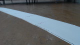
\includegraphics[width=0.31\textwidth]{imgs/sample_left.png}
  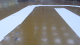
\includegraphics[width=0.31\textwidth]{imgs/sample_up.png}
  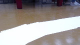
\includegraphics[width=0.31\textwidth]{imgs/sample_right.png}
  \caption{Sample images from training dataset.\label{fig:dataset_sample}}
\end{figure}

\autoref{fig:dataset_sample} showcases sample images from the training dataset. The leftmost image
has label $\Left$, the one on the middle is $\Up$ and the one on the right $\Right$. It is possible
to observe that images do not have uniform lightning and lane markings are irregular. This adds a
noise effect to the images.

The original dataset is already reduced in size. However, the presence of color is not so important
to identify the correct values of $Y$. If we compare~\autoref{fig:dataset_sample}
and~\autoref{fig:dataset_gray}, lane markings are still very much visible.

\begin{figure}[h]
  \centering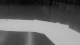
\includegraphics[width=0.31\textwidth]{imgs/gray_left.png}
  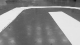
\includegraphics[width=0.31\textwidth]{imgs/gray_up.png}
  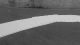
\includegraphics[width=0.31\textwidth]{imgs/gray_right.png}
  \caption{Grayscale sample images from training dataset.\label{fig:dataset_gray}}
\end{figure}

We can try to further reduce the complexity of the dataset at the same time preserving its most
informational features by attempting to reduce the number of possible values of each pixel through
image quantization. This transformation turned out to be very meaningful in terms of both training
speed and accuracy, as we detail in a later chapter. However, noise is still very much present in
the images, as~\autoref{fig:dataset_transformed} shows.

\begin{figure}[h]
  \centering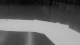
\includegraphics[width=0.31\textwidth]{imgs/trans_left.png}
  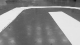
\includegraphics[width=0.31\textwidth]{imgs/trans_up.png}
  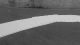
\includegraphics[width=0.31\textwidth]{imgs/trans_right.png}
  \caption{Quantized sample images from training dataset.\label{fig:dataset_transformed}}
\end{figure}

Another possible transformation we can apply on the dataset is binarization. However, traditional
``hard'' binarization with a fixed $k$ threshold on the image could potentially cause completely
black or white images due to a poor choice of $k$. This can countered with two possible solutions.
Either through adaptive threshold where we choose $k$ either by a mean measurement or through a
gaussian, or by use of Otsu's binarization (\cite{otsu}). We found that Otsu's method, coupled with
a prior gaussian blur transformation on each image, proved the most capable of correctly applying
binarization in our dataset.

\begin{figure}[h]
  \centering
\includegraphics[width=0.31\textwidth]{imgs/binary_left.png}
  
\includegraphics[width=0.31\textwidth]{imgs/binary_up.png}
  
\includegraphics[width=0.31\textwidth]{imgs/binary_right.png}
  \caption{Binarized sample images from training dataset.\label{fig:dataset_binary}}
\end{figure}

\autoref{fig:dataset_binary} shows the final result of applying a combination of gaussian blur and
Otsu's binarization.

One last transformation we tested our models on was histogram equalization. Equalization was done
in order to reshape the pixel value histogram to an approximately uniform distribution. This was
done in an attempt to increase the accuracy of the Gens-Domingos algorithm. As mentioned
in~\autoref{chp:structure}, the Gens-Domingos schema attempts to find partitions of independent
variables. We use an implementation of the G-test, which works best when there are sufficient
samples for every variable category. The original dataset has a skewed histogram that contains
almost no pixel values in the extreme ranges (either too white or too black). This transformation
added a lot of noise to the dataset. In spite of this, we empirically found that with the use of
equalization accuracy was increased by more or less 5\%.

\begin{figure}[h]
  \centering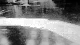
\includegraphics[width=0.31\textwidth]{imgs/eq_left.png}
  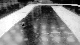
\includegraphics[width=0.31\textwidth]{imgs/eq_up.png}
  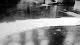
\includegraphics[width=0.31\textwidth]{imgs/eq_right.png}
  \caption{Equalized sample images from training dataset.\label{fig:dataset_equalized}}
\end{figure}

\section{The model}

Our classification model should be able to accurately infer the most probable action to be taken
given the front camera feed's image. Although a simple decision model could be used for such a
task, in many cases we wish to maintain an uncertainty measurement (e.g. a probability
distribution) as a means to quantify error. Error and noise is often a problem in robotics, one
which can be mitigated through probabilistic localization algorithms. For our particular case, we
discard these problematic issues and focus solely on the problem of computing a valid probability
distribution that accurately models our classification problem. SPNs have full probabilistic
semantics and are able to represent local and sparse variable interactions due to their deep
architecture. This allows for a reliable probabilistic model for modelling our classification
problem.

We use two SPN architectures for our problem. We model the first using the Dennis-Ventura algorithm
described in~\autoref{section:dv}. This model in particular uses the classification architecture
also cited in~\autoref{chp:structure}. The second model uses the Gens-Domingos structural algorithm
(\autoref{section:gd}).

As we have previously mentioned, we wish to compute the MPE

\begin{equation}
  \argmax_{y\in\Val(Y)} P(Y=y,X)=\argmax_{y\in\Val(Y)}S(Y=y,X)\approx y|_{M(Y=y,X)}, y\in\Val(Y).
\end{equation}

Where $y|_{M(Y=y,X)}$ signals an MPN forward and backward pass to compute the most probable
explanation of variable $Y$ given $X$ as evidence on the underlying SPN.

Recalling~\autoref{chp:spn}, we can compute this probability in two different ways. Either
by computing each $Y$ value by means of a forward pass on the SPN $S(Y=y,X)$, or through the
approximate MAP $M(Y=y,X)$. These two options both carry disadvantages. On one hand, computing each
$Y$ value through a forward pass on each possible valuation can cause inference to become very
slow, especially when hardware is as limited as in a mobile robot. On the other hand, the
max-product algorithm is a fast inference method, though approximate. Furthermore, the approximate
method tends to favor shallower paths due to its Viterbi-style features.

We compromise with exact inference, but with an addendum. We take advantage of our hardware's
multi-cored CPU by running exact inference in parallel. Since the Gens-Domingos and Dennis-Ventura
architectures are very distinct structure-wise, we apply a different implementation for each.

As mentioned in~\autoref{chp:structure}, the Dennis-Ventura structure we implemented follows a
particular classification architecture that models each set of images of a certain label as a
separate, independent sub-SPN. This allows for an easy parallel programming implementation, as each
CPU core can be assigned to a single sub-SPN, and thus to a label. Each core will then be linked to
a particular robot command. Once all cores finish inference, we then compare which sub-SPN returned
the highest probability. This is only advantageous if the number of labels is low. In our case,
$|\Val(Y)|=3$, meaning this method is feasible for our problem.

This method does not work as well on the Gens-Domingos structure, as we cannot guarantee if
an independency or clustering step on the root node has yielded a sufficient number of nodes for
each core. However, a similar method is used, where a concurrency queue of $n$ most processes
stores each child of the root node, allowing for them to be run in parallel. Since the
Gens-Domingos structural algorithm produces SPTs, every child of a node is guaranteed to be
independent of its siblings.

